
\documentclass[12pt,a4paper]{report}
\usepackage[T1]{fontenc}
%\usepackage[utf8]{inputenc}
\usepackage{amsmath}
\usepackage{amsfonts}
\usepackage{amssymb,lipsum,natbib,color,verbatim}
\usepackage{graphicx}
\DeclareMathOperator{\cosec}{cosec}

\author{\color{red}Chandra Has\\ \scriptsize chandrahashbti@gmail.com}
\title{\color{blue}\textbf{Tips and Tricks in \LaTeX}}

\begin{document}
\maketitle

\section*{Important points:}
\begin{enumerate}
 \item New para:\\
$\verb|\\, \par, blank line (recommended)|$
\item Little extra space:\\
$I = \int e^x\,dx $ \hfil  \checkmark\\
$I = \int e^xdx $ \hfil  $\times$
\item Align (recommended) vs eqnarray 
\item Functions name:\\
$\log, \ln, \sin, \cos, \tan,\cosec^*, \exp$  \hfil  \checkmark\\
$log, ln, sin, cos, tan, cosec, exp$\hfil  $\times$\\
*declared math operator
\item Dots: \\
As mentioned\ldots\hfil  \checkmark\\
As mentioned... \hfil  $\times$
\item Page ranges:\\
--\hfil  \checkmark\\
- \hfil  $\times$
\item Avoid to use: \\
\verb|\newpage, \bigskip, \medskip, smallskip,|\\
\verb|\pagebreak, \linebreak|
\item Cross referencing command:\\
\verb|\ref{}, \eqref{}, \pageref{},|\\
\verb|\cref{}, \Cref{}, \crefrange{}, \Crefrange{}|
\item Displaymath:\\
\verb|$$---$$, \[\]|(recommended)
\item Angled bracket 
\item Delimiters size\\
\verb|\left[...\right], \left(...\right), \left\{\right\}|,\\
\verb|\big, \bigg, \biggr, \biggm, \biggl, \Big, \Bigg, \Biggl, \Biggm, \Biggr|,\\
e.g. $\left[\frac{e^e - 1}{\ln(100)} + 6\right]$,
$\Big[\frac{e^e - 1}{\ln(100)} + 6\Big]$, $\Big\vert$
\item Uppercase in references: \verb|{Letter}|
\item Inverted commas:\\
load \verb|\usepackage{csquote}|  package in the preamble and use \verb|\enquote{---}|\\ 
 or from the keyboard\\
{\centering
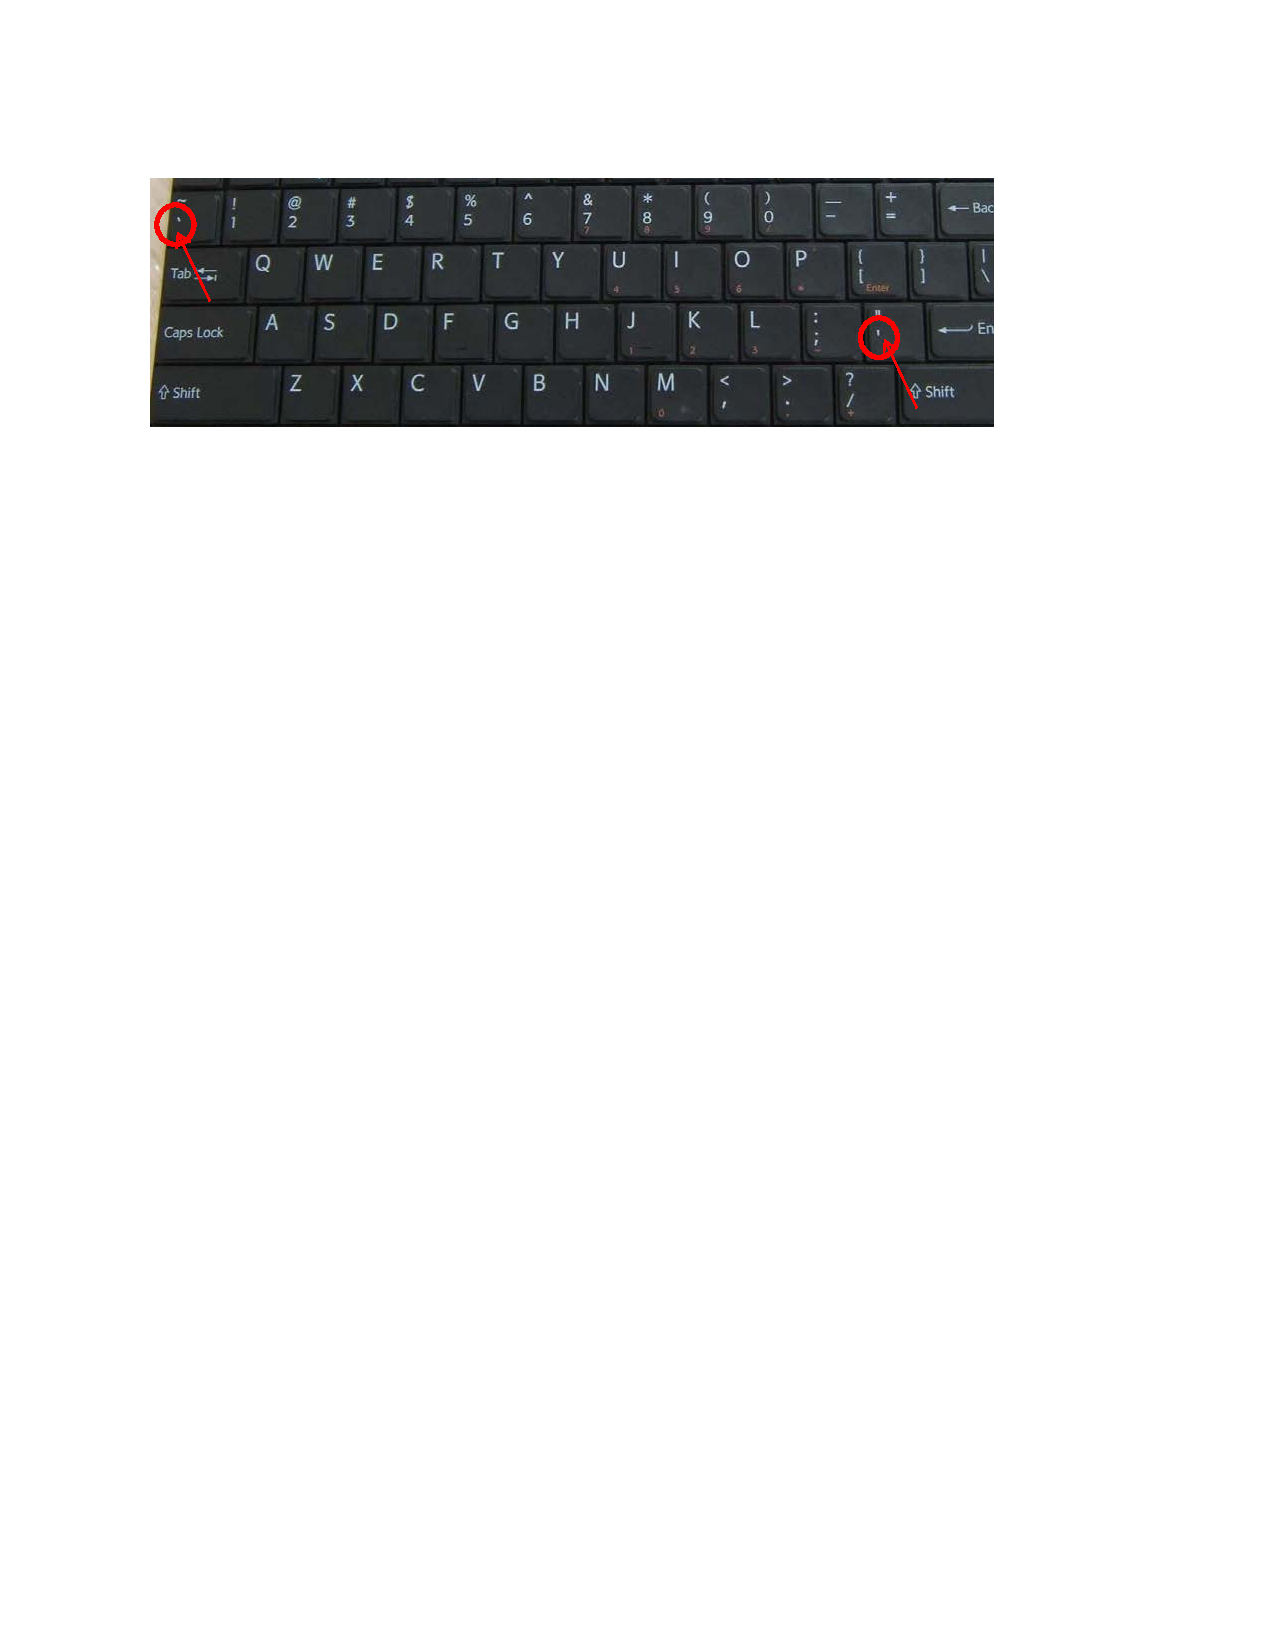
\includegraphics[width=1\textwidth]{keyboard}}
\item Order of packages
\item Add extra line:
\verb|\enlargethispage{number\baslineskip}| 
\item Clean auxiliary files
\end{enumerate}
\section*{Common errors:}
\begin{enumerate}
\item ! Extra \verb|}  or forgotten $| \\
$\Rightarrow$ check \verb|{each}| and \verb|$each$|
\item ! Emergency stop \\
missing  \verb|\end{document}| or wrong spelling
\item ! I can't write on file ` ' \\
Close opened pdf (specially in Acrobat)
\item ! Paragraph ended before ... was complete\\
wrong command name e.q.\verb| \smalll|,\\
missing \verb|}|
\item ! Too many \verb|}|'s\\
missing \verb|{|
\item ! Undefined control sequence\\
command name is not spelled correctly
\item ! Missing \verb|$| inserted\\
\verb|$---$, or \begin{math}---\end{math} or \ensuremath{---}|
\item ! LaTeX Error: File `name.sty' not found\\
misspelled package name,\\
download required package first and put it in the same folder
\item ! LaTeX Error: Option clash for package\\
change the order of package,\\
remove the option
\item ! LaTeX Error: Missing \verb|\begin{document}|\\
Avoid to type any printable text in the preamble
\item ! File ended while scanning use of \verb|\end|\\
May be you have not closed something properly, e.g. forgot to use \verb|}|
\end{enumerate}

\clearpage
\lipsum[1-4]
\enlargethispage{1\baselineskip}
Contrary to popular belief, Lorem Ipsum is not simply random text. It has roots in a piece of classical Latin literature from 45 BC, making it over 2000 years old. Richard McClintock, a Latin professor at Hampden-Sydney College in Virginia, looked up one of the more obscure Latin ordsContrary to popular belief, Lorem Ipsum is not simply random text. 

%Contrary to popular belief, Lorem Ipsum is not simply random text. It has roots in a piece of classical Latin literature from 45 BC, making it over 2000 years old. Richard McClintock, a Latin professor at Hampden-Sydney College in Virginia, looked up one of the more obscure Latin ordsContrary to popular belief, Lorem Ipsum is not simply random text. 

\section*{Document Structure}
\begin{verbatim}
\RequirePackage[l2tabu]{nag}
% % % % % % % % % % % % % % % % % % % % % % % % % % % % % % % % % %

% % % % % % % % % % %Packages % % % % % % % % % % % % % % % % %
% % % % % % % % % % % % % % % % %Chandra Has % % % % % % % % % % % %

% % % % % % % % % % % %chandrahashbti@gmail.com % % % % % % % %

\documentclass[12pt,a4paper,twoside,openright]{report}

% % % % Fonts type and spacing % % % % % % % % %
\usepackage[T1]{fontenc}
\usepackage[english]{babel}
\usepackage[sc]{mathpazo}
\linespread{1.05} % Palatino needs more leading (space between lines)
%\usepackage{times}
%\usepackage{mathptmx}
%\usepackage[varg]{txfonts}
\usepackage[onehalfspacing]{setspace}

% % % % AMS packages % % % % % % % % % % % % % % % %
\usepackage{amsmath}
\usepackage{amssymb}         
\usepackage{amsfonts}

% % % % Layout % % % % % % % % % % % % % % % % % % %
\usepackage{geometry}
\geometry{ %
 a4paper,
 total={210mm,297mm},
 inner=3.5cm,
 outer=2.5cm,
 top=2.5cm,
 bottom=2.5cm,
 }
%\usepackage{anysize}
%\marginsize{3.5cm}{2.5cm}{2.5cm}{2.5cm}
\usepackage[stretch=10,shrink=10]{microtype}
\usepackage{fancyhdr}
 \pagestyle{fancy} 
\usepackage{emptypage} 
%emptypage:to Remove haeader from the blank page in twosided layout
\usepackage{afterpage}
\usepackage{ragged2e} %\justifying
\usepackage{quotchap}
  \qsetcnfont{pnc}
%\usepackage[Sonny]{fncychap}
%\usepackage{background}
% \backgroundsetup{contents=Draft,scale=4,position={2,-3.5},opacity=1}
\usepackage{fancybox}
 \raggedbottom
% \raggedbottom : No extra vertical space is added. 

% % % % % % % % % Graphics % % % % % % % % % % % %
\usepackage[demo]{graphicx}
%\graphicspath{{image1/}{image2/}}
\usepackage{float}
\usepackage{grffile} %grffile is used to allow spaces in images in pdfTeX
\usepackage{caption}
 %\captionsetup{font={small, singlespacing}, justification=justified}
\usepackage{subcaption}

% % % % % % % Lists % % % % % % % % % % % % % % % %
\usepackage[intoc]{nomencl}
  \makenomenclature
\usepackage[round]{natbib}
\usepackage[toc,page]{appendix}
%\usepackage{chapterbib}
\usepackage{tocbibind}
%\usepackage[undotted]{minitoc}

% % % % Title % % % % % % % % % % % % % % % % % % %
\usepackage{titletoc}
\usepackage[toctitles]{titlesec}
%\usepackage{tocloft}
%\usepackage{titlepage}

% % % % Misc % % % % % % % % % % % % % % % % % % %
\usepackage{bm}
\usepackage{enumerate}
\usepackage[version=3]{mhchem}
\usepackage{booktabs}
\usepackage{array}
\usepackage{longtable}
\usepackage{multirow}
\usepackage{calc}
\usepackage{cancel}
\usepackage{vector}
\usepackage{soul}
\usepackage{colonequals}
\usepackage[normalem]{ulem}
\usepackage{ifthen}
\usepackage{etoolbox}
\usepackage{empheq}
\usepackage{color}
\usepackage[table]{xcolor}
\usepackage{multirow}
\usepackage[bottom]{footmisc}
\usepackage{numprint}
\usepackage[allowlitunits]{siunitx}
\usepackage{nicefrac}
\usepackage{xfrac}
\usepackage{theorem}
\usepackage{listings}
\usepackage{lscape}
\usepackage{xspace}
\usepackage{commath}
\usepackage{vector}
\usepackage{tensor}
\usepackage{eucal}
\usepackage[euler]{textgreek}
\usepackage[Euler]{upgreek}
\usepackage{filecontents}
\usepackage[nomargin,footnote,index]{fixme}
\usepackage{hyphenat} 
\usepackage{csquotes}
\usepackage{lipsum}
\usepackage{verbatim}
\usepackage{filecontents}
\usepackage{hyperref}
 \hypersetup{
     bookmarks=true,         % show bookmarks 
     unicode=false,          % non-latin characters in Acrobat's bookmarks
     pdftitle={Ch},          % title
     pdfauthor={Chandra Has},% author
     pdfnewwindow=true,      % links in new window
     colorlinks=true,        % false: boxed links; true: colored links     
     citecolor=blue,         % color of links to bibliography
     urlcolor=green          % color of external links
 }
 
 % % %Packages must be loaded after hyperref % % % % %
\usepackage[capitalise]{cleveref}
\usepackage{algorithm}
\usepackage{bookmark}
\usepackage[toc]{glossaries}
  \makeglossaries
\usepackage{imakeidx}
  \makeindex[title=Index 1]
%  \makeindex[name=p,title=Index 2]

% % % Customm commands % % % % % % % % % % % % % % % % % %
\definecolor{chaptergrey}{rgb}{.5 .5 .5}
\newcommand{\printpageintoc}{\addtocontents{toc}{~\hfill\textbf{Page}\par}}
% \printpageintoc works with "afterpage" package 

\renewcommand{\bibname}{References}

\begin{document}

\thispagestyle{empty}
\include{Title}

\cleardoublepage
\phantomsection
\pagestyle{plain}
\pagenumbering{roman}
\addcontentsline{toc}{chapter}{Abstract}
\include{Abstract}

\cleardoublepage
\phantomsection
\include{Dedication}

\cleardoublepage
\phantomsection
\include{Declaration}

\cleardoublepage
\phantomsection
\include{Acknowledgements}

\cleardoublepage
\phantomsection
\printnomenclature

\cleardoublepage
\phantomsection
\printpageintoc
\tableofcontents

\cleardoublepage
\phantomsection
\listoffigures

\cleardoublepage
\phantomsection
\listoftables

\cleardoublepage
\phantomsection
\pagestyle{fancy}
\pagenumbering{arabic}
\setcounter{page}{1}
\include{chap01}
\include{chap02}
  
\cleardoublepage
\phantomsection
\addcontentsline{toc}{chapter}{References}
\bibliographystyle{apalike}
\bibliography{mybib}

\cleardoublepage
\phantomsection
\appendix
\include{app01}

 \end{document}  
%%--------------------------------------------------- % %
\end{verbatim}



\bibliographystyle{chicago}
\bibliography{tips}
\nocite{*}

\end{document}